\section{Origen de la filosofía lean}

\subsection{Primeros avances de la gestión Lean}

Los primeros desarrollos de las herramientas lean se remontan a los primeros tiempos de la industrialización.
Con el aumento de la demanda de los clientes, los empresarios intentaban implantar procesos que aceleraran y aumentaran la producción.
Eli Whitney, se hizo famosos por ser el inventor de la desmotadora de algodón.
Sin embargo, la desmotadora fue un logro menor comparado con su perfección de las piezas intercambiables.
Whitney lo desarrolló hacia 1799, cuando aceptó un contrato del ejército estadounidense para la fabricación de 10.000 mosquetes a un precio realmente bajo de 13 dólares por cada arma.

Durante los 100 años siguientes, los fabricantes se ocuparon principalmente de tecnologías individuales.
Durante este tiempo se desarrolló el sistema de planos de ingeniería, se perfeccionaron las máquinas-herramienta modernas y los procesos a gran escala, como el proceso Bessemer para fabricar acero, ocuparon el centro de atención.
Mientras los productos pasaban de un proceso discreto al siguiente a través del sistema logístico y dentro de las fábricas, poca gente se preocupaba por:

\begin{itemize}
    \item Qué ocurre entre un proceso y otro
    \item Cómo se organizaron los múltiples procesos dentro de la fábrica
    \item Cómo funcionaba la cadena de procesos como sistema
    \item Cómo realizó una tarea cada trabajador
\end{itemize}

\subsection{Ford y el Taylorismo}

Esto cambió a finales de la década de 1890 con el trabajo de los primeros ingenieros industriales.
Frederick W. Taylor empezó a estudiar a cada trabajador y sus métodos de trabajo.
El resultado fueron los estudios sobre la gestión del tiempo, el tiempo por ciclo y las operaciones de trabajo estandarizadas.
Llamó a sus ideas gestión científica \cite{hounshell_same_1988}.
Taylor fue un directivo con una personalidad controvertida.
El concepto de aplicar la ciencia a la gestión era sólido, pero Taylor simplemente ignoró las ciencias del comportamiento.
Además, tenía una actitud peculiar hacia los trabajadores de las fábricas.
Frank Gilbreth añadió el estudio del movimiento e inventó los gráficos de procesos.
Los gráficos de procesos centraban la atención en todos los elementos del trabajo, incluidos los elementos sin valor añadido que normalmente se producen entre los elementos "oficiales".

Lillian Gilbreth introdujo la psicología al estudiar las motivaciones de los trabajadores y cómo las actitudes afectaban al resultado de un proceso.
Hubo, por supuesto, muchos otros colaboradores.
Estas personas fueron las que originaron la idea de "eliminar los residuos", un principio clave del JIT y la fabricación ajustada.
Aunque existen ejemplos de procesos de fabricación rigurosos que se remontan al Arsenal de Venecia en la década de 1450, la primera persona que integró realmente todo un proceso de producción fue Henry Ford.
En 1913, en Highland Park (Michigan), unió las piezas intercambiables con el trabajo estándar y el transporte en movimiento para crear lo que denominó "producción en cadena"
El público lo entendió en la dramática forma de la cadena de montaje en movimiento, pero desde el punto de vista del ingeniero de fabricación, los avances en realidad iban mucho más allá.

Ford alineaba los pasos de fabricación en la secuencia del proceso siempre que era posible, utilizando máquinas especiales y calibradores \textit{poka-yoke} para fabricar y ensamblar los componentes del vehículo en pocos minutos y entregar los componentes perfectamente ajustados directamente a la línea de producción.
Se trataba de una ruptura verdaderamente revolucionaria con respecto a las prácticas de taller del sistema americano, que consistía en máquinas de uso general agrupadas por procesos, que fabricaban piezas que acababan convirtiéndose en productos acabados tras un buen rato de retoques en el subensamblaje y el ensamblaje final.
El problema del sistema de Ford no era el flujo ya que era capaz de dar la vuelta a los inventarios de toda la empresa cada pocos días.
Más bien era su incapacidad para ofrecer variedad.

El Modelo T no sólo se limitaba a un color, que era negro. También se limitó a una especificación, de modo que todos los chasis del Modelo T eran esencialmente idénticos hasta el final de la producción en 1926.
El cliente sí podía elegir entre cuatro o cinco estilos de carrocería, una característica añadida por proveedores externos al final de la línea de producción.
De hecho, parece que prácticamente todas las máquinas de la Ford Motor Company trabajaban con un único número de pieza, y prácticamente no había cambios.
Cuando el mundo quiso variedad, incluyendo ciclos de modelos más cortos que los 19 años del Modelo T, Ford pareció perder el rumbo.

Otros fabricantes de automóviles respondieron a la necesidad de muchos modelos, cada uno con muchas opciones, pero con sistemas de producción cuyos pasos de diseño y fabricación retrocedían hacia áreas de proceso con tiempos de producción mucho más largos.
Con el tiempo, poblaron sus talleres de fabricación con máquinas cada vez más grandes que funcionaban cada vez más rápido, lo que aparentemente reducía los costes por paso del proceso, pero aumentaba continuamente los tiempos de producción y los inventarios, excepto en algunos casos (como las líneas de mecanizado de motores) en los que todos los pasos del proceso podían conectarse y automatizarse \cite{hounshell_same_1988}.
Peor aún, los desfases entre las fases del proceso y las complejas rutas de las piezas exigían sistemas de gestión de la información cada vez más sofisticados, que culminaron en los sistemas informatizados de planificación de necesidades de materiales (MRP).

\subsection{Sistema de Producción Toyota (TPS)}

Cuando Kiichiro Toyoda, Taiichi Ohno y otros miembros de Toyota analizaron esta situación en década de 1930, y más intensamente justo después de la II Guerra Mundial, se les ocurrió que una serie de una serie de sencillas innovaciones podría hacer más posible la continuidad continuidad en el flujo de procesos y una amplia variedad en la oferta de productos.
Así pues, retomaron Ford e inventaron el sistema de producción Toyota.

En esencia, este sistema desplazó la atención del ingeniero de fabricación de las máquinas individuales y su utilización al flujo del producto a través del proceso total.
Toyota llegó a la conclusión de que si se ajustaba el tamaño de las máquinas al volumen real necesario, se introducían máquinas con autocontrol para garantizar la calidad, se alineaban las máquinas en la secuencia del proceso, se iniciaban configuraciones rápidas para que cada máquina pudiera fabricar pequeños volúmenes de muchos números de piezas y se hacía que cada paso del proceso notificara al paso anterior sus necesidades actuales de materiales, sería posible obtener bajos costes, alta variedad, alta calidad y tiempos de producción muy rápidos para responder a los deseos cambiantes de los clientes.
El concepto del TPS se basa en un paradigma de mejora permanente y continua, la filosofía kaizen.
Además, la gestión de la información podría ser mucho más sencilla y precisa \cite{liker_toyota_2006}.
En el libro \textit{La Máquina Que Cambió el Mundo} \cite{womack_machine_2007}, se describe detalladamente el proceso de pensamiento del lean.
En él los autores describen que los principios del lean se basan en cinco elementos:

\begin{itemize}
    \item Especificar el valor deseado por el cliente.
    \item Identificar el flujo de valor de cada producto que aporta ese valor y cuestionar todos de los pasos desperdiciados necesarios actualmente.
    \item Hacer que el producto fluya continuamente a través de las etapas de valor añadido.
    \item Introducir tirones entre todos los pasos en los que sea posible un flujo continuo.
    \item Perfeccionar el proceso para que el número de pasos y la cantidad de tiempo e información necesarios para atender al cliente disminuyan continuamente.
\end{itemize}

\subsection{La gestión Lean en la actualidad}

Este éxito continuado ha generado en las dos últimas décadas una enorme demanda de conocimientos sobre el pensamiento lean.
Hay literalmente cientos de libros y documentos, por no hablar de los miles de artículos de los medios de comunicación que exploran el tema, y otros muchos recursos a disposición de este público cada vez más numeroso.
A medida que el pensamiento lean sigue extendiéndose por todos los países del mundo, los líderes también están adaptando las herramientas y los principios más allá de la fabricación, a la logística y la distribución, los servicios, el comercio minorista, la sanidad, la construcción, el mantenimiento e incluso la administración pública.

De hecho, la conciencia y los métodos lean están empezando a arraigar entre los altos directivos y líderes de todos los sectores en la actualidad.
Las redes de cadenas de valor en los tiempos actuales son estructuras complejas e internacionales de oferta y demanda \cite{helmold_global_2016}.
Especialmente, los fabricantes japoneses muestran cómo los proveedores se integran de forma sostenible en la propia cadena de valor y actividades \cite{lincoln_keiretsu_1992}.
Las redes japonesas se describen como redes \textit{keiretsu}, en las que proveedores y clientes son sistemas integrados a lo largo de la cadena de valor.
En el futuro, la competitividad se decidirá en función de quién tenga la red de valor más flexible y eficiente, que incluya flujos de valor desde los proveedores de materias primas, pasando por las operaciones propias, hasta la distribución a los clientes \cite{singh_srai_supply_2008}.

\section{Estandarización}

Existe una interpretación errónea, muy extendida y originada por los consultores, del concepto de trabajo normalizado.
El objetivo principal del trabajo normalizado no es tener definidos los procedimientos normalizados de trabajo ni disponer de una línea de base para el enfoque PDCA de mejora continua (ciclo Planificar-Hacer-Verificar-Actuar de Deming); esto puede ser un beneficio secundario derivado y bienvenido.
Sin embargo, el trabajo normalizado es fundamental para implantar el flujo de pieza única (SPF) en las células de trabajo. Podemos definir el trabajo normalizado del siguiente modo:

\begin{quote}
    El trabajo normalizado es la combinación óptima de operarios, máquinas y material para garantizar que una tarea se realiza siempre de la misma manera con el mínimo desperdicio para cumplir sistemáticamente el \textit{tack time}.
    El trabajo normalizado se compone de los elementos \textit{tack time}, contenido del trabajo (WC), secuencia de trabajo WIP estándar y personal adecuado.
    El trabajo normalizado debe ser definido, mantenido y mejorado por los operarios y los supervisores.
\end{quote}

De hecho, en una célula de modelo mixto de SPF programado y tomado de la caja Heijunka, es decir, una célula de trabajo dedicada a múltiples productos similares pero diferentes, es de suma importancia que PLT y ER satisfagan la demanda de reabastecer a tiempo el supermercado controlado por Kanban para evitar que se agoten las existencias.
Para ello, el trabajo de los operarios debe ser repetible y reproducible.
Herramientas útiles en este contexto son las \textbf{Tablas de Capacidad de Proceso} y las \textbf{Tablas de Combinación de Trabajo Estandarizadas}. No entraremos aquí en el amplio e interesante tema del diseño de células industriales, con los conceptos adicionales de estación de trabajo (WTT) y tiempo de rotación de células (CTT), sino que intentaremos transponer parte de la técnica al contexto de la oficina.

En el contexto industrial, el cronómetro es una herramienta esencial para realizar un trabajo normalizado. Es obligatorio medir el tiempo de ciclo de las tareas, incluso de cada uno de los pasos. No sólo para mejorar la línea de base, sino también para poder planificar y aplicar la célula. Para ello, el contenido del trabajo lo define y ejecuta el mejor operario, cuyo ritmo deben alcanzar todos los demás operarios. Se definen las entidades de actividad lógica como:

\begin{itemize}
    \item Paso
    \item Tarea
    \item Subproceso
    \item Proceso principal
\end{itemize}

Debido a la diferencia intrínseca de una transacción en comparación con un producto, en una transacción cada nuevo pedido es diferente, incluso en la misma categoría de productos, lo que se aproxima a un tamaño de lote real 1 para cada transacción.
Debido a esta característica, las entidades de actividad "paso" y "tarea" pueden presentar un contenido variable y, por lo tanto, un tiempo de ciclo variable; por ejemplo, la concesión de un crédito bancario puede depender de factores contingentes para los que se necesite más tiempo.
Por lo tanto, es recomendable, al menos al principio, dejar cierta discrecionalidad al empleado definiendo un límite superior para ejecutar una tarea o incluso definir el PLT máximo aceptable para una rutina definida, límite superior que, por supuesto, puede ser cuestionado por el supervisor.
En efecto, aunque también, por ejemplo, las entidades de crédito hablan de productos, el contenido de los productos es muy variable y difiere de un pedido a otro.
Por lo tanto, tiene más sentido hablar del producto en las industrias de servicios como una plantilla paramétrica con una estructura definida pero con un contenido variable.
Con cada pedido, el contenido tiene que rellenarse en la estructura de la plantilla para luego ser procesado.
Esta es la razón por la que preferimos no hablar de trabajo estandarizado en el entorno de oficina, que implica una estricta observación del tiempo para cada paso (porque se ejecuta en células de alto rendimiento), sino que preferimos hablar de trabajo normalizado, que permite cierta discrecionalidad en la ejecución de la rutina.

Definamos el trabajo normalizado como un "estándar de trabajo contingente" para completar una tarea en un plazo determinado de acuerdo con un PNT definido.
Es preferible hablar de trabajo normalizado (en un entorno de oficina) en lugar de trabajo estandarizado (industria) debido al contenido de transacción no determinista en comparación con el contenido de trabajo determinista de un producto industrial.
Por lo tanto, el enfoque debería cambiar del tiempo de ciclo de una tarea al tiempo de transacción de un subproceso, ya que el contenido no determinista conduce a una "ejecución normalizada" por transacción.
Sin embargo, también para la transformación de pedidos basada en transacciones, el cronómetro y las mediciones de tiempo pueden registrarse utilizando un gráfico de observación del tiempo de proceso. Los registros repetitivos ayudan a estratificar los productos en categorías, por ejemplo, sencillos, medianos, complejos, que tardan distinto tiempo en procesarse.

Tenga en cuenta que la suma de las tareas corresponde al contenido del trabajo (WC).
Si las tareas se ejecutan sin interrupción, es decir, sin tiempo de espera entre ellas, el WC corresponde también a la rutina PLT.
Si durante la rutina una tarea necesita la intervención de otro departamento, el tiempo de espera es la consecuencia y puede acumularse un WIP.
En ese caso, el PLT de la rutina debe tener en cuenta este tiempo de espera; una alternativa es dividir la rutina en una parte y una parte separadas por el WIP.
Esto es recomendable si el tiempo de espera es largo con respecto al WC o si las dos partes funcionan a un ritmo diferente; esto permite cambiar a otra actividad mientras tanto.

Debido a la diferencia intrínseca entre la fabricación y la oficina -recordemos que, debido al contenido paramétrico de una orden transaccional, es difícil prescribir el tiempo de una secuencia de pasos individuales dentro de una tarea en un PNT detallado-, no hay que prescribir la secuencia temporal exacta, sino en qué plazo debe entregarse el resultado.
Por supuesto, si los tiempos pueden variar, el PLT del procedimiento, subrutina o proceso, variará, pero no debe variar demasiado, ni entre empleados.
Para limitar la discrecionalidad del empleado es posible definir clases dentro de un tipo de producto realizado en la misma rutina, por ejemplo, transacciones simples, transacciones de tiempo medio absorción, y transacciones complejas.

Por supuesto, esto conduce a una PLT variable de la misma rutina, pero la variabilidad no se debe a la no repetibilidad o no reproducibilidad de la orden, sino al contenido variable del mismo tipo de órdenes. En efecto, como ya hemos visto en el Cap. 2, debido al hecho de que el rendimiento de un servicio se determina "paramétricamente" a través de la unicidad de cada especificación de orden, no podemos hablar de una "repetibilidad idéntica" (y reproducibilidad) de las órdenes, sin embargo, como mucho podemos hablar de una "repetibilidad formal" (y reproducibilidad) que se refiere a la repetición del proceso pero no al contenido.

Y precisamente esta falta de "repetibilidad idéntica" y de "reproducibilidad idéntica", en la mayoría de los procesos, nos conducirá hacia una modelización diferente del trabajo de oficina en comparación con el trabajo de fabricación: una más parecida a la forma (funcional y relacional en lugar de procedimental), pero también definida por el objetivo en lugar de por un algoritmo determinista.
Por tanto, el PNT tiene más bien el carácter de una lista de comprobación.

Al principio de esta sección decíamos que el trabajo normalizado no es sinónimo de procedimiento operativo normalizado (PNT); de hecho, el PNT puede ser una aportación para definir el trabajo normalizado.
Sin embargo, los PNT también son importantes en la oficina para garantizar la reproducibilidad formal de los procesos por parte de los empleados cualificados.
Los PNT deben ser fáciles de leer y utilizar listas de comprobación; estos PNT ayudan también a los empleados principiantes a familiarizarse rápidamente con la gestión reproducible de las transacciones.
Debido a que las transacciones se realizan a menudo mediante la división del trabajo que implica a diferentes empleados que necesitan reuniones, los PNT sobre cómo dirigir o participar en las reuniones son de suma importancia para que el resultado sea lo más eficaz posible.
Aunque este tema es muy importante no entramos más en este debate.

Para aproximar la "repetibilidad formal" a una "repetibilidad idéntica" (así como la reproducibilidad, por supuesto) es necesario definir una estratificación dentro del producto, que corresponde a una mezcla de productos, lo que permite planificar mejor la carga de un equipo, es decir, la célula de oficina, y controlar la eficacia del equipo.
Aunque pueda parecer extraño aplicar un método de trabajo basado en el tiempo en el mundo de la oficina, el aumento de la competencia global obliga a la dirección a aplicar métodos de aumento de la productividad probados en la industria también para las transacciones del entorno de oficina, independientemente de si se trata de front office o back office.
Sin embargo, la aplicabilidad de normas estrictas de tiempo debido a la variabilidad del contenido de los pedidos es difícil, como acabamos de ver.
Por tanto, es importante especificar límites superiores de especificación (USL) para el TC, concepto derivado de la teoría de la capacidad de Seis Sigma, no sólo para cada producto, sino también para cada categoría de estratificación dentro de cada producto, y supervisar la estabilidad del proceso con gráficos de control de Seis Sigma.

\section{Estándar BPMN}

El Business Process Model and Notation (BPMN) se encuentra entre los lenguajes de modelado de procesos y decisiones más extendidos.
Su objetivo es proporcionar a los usuarios empresariales modelos de gran comprensión, que también puedan utilizarse para su aplicación.
En función del objetivo del modelado, los modelos de procesos presentan diferentes niveles de abstracción con respecto al proceso empresarial subyacente.
En un nivel organizativo, se da la descripción textual de alto nivel de un proceso, incluyendo las entradas, salidas y responsabilidades del proceso.
Un modelo de proceso operativo captura las actividades, su relación, así como la información organizativa.
El nivel operativo está subdividido por BPMN, en modelos descriptivos, para una documentación de alto nivel, y modelos analíticos, para analizar el proceso en detalle.
A partir de ahí, un modelo de proceso implementado lo amplía y adapta con los aspectos técnicos necesarios para la implementación.

Esta sección pretende presentar rápidamente el estándar BPMN con un ejemplo clínico.

\begin{figure}
    \centering
    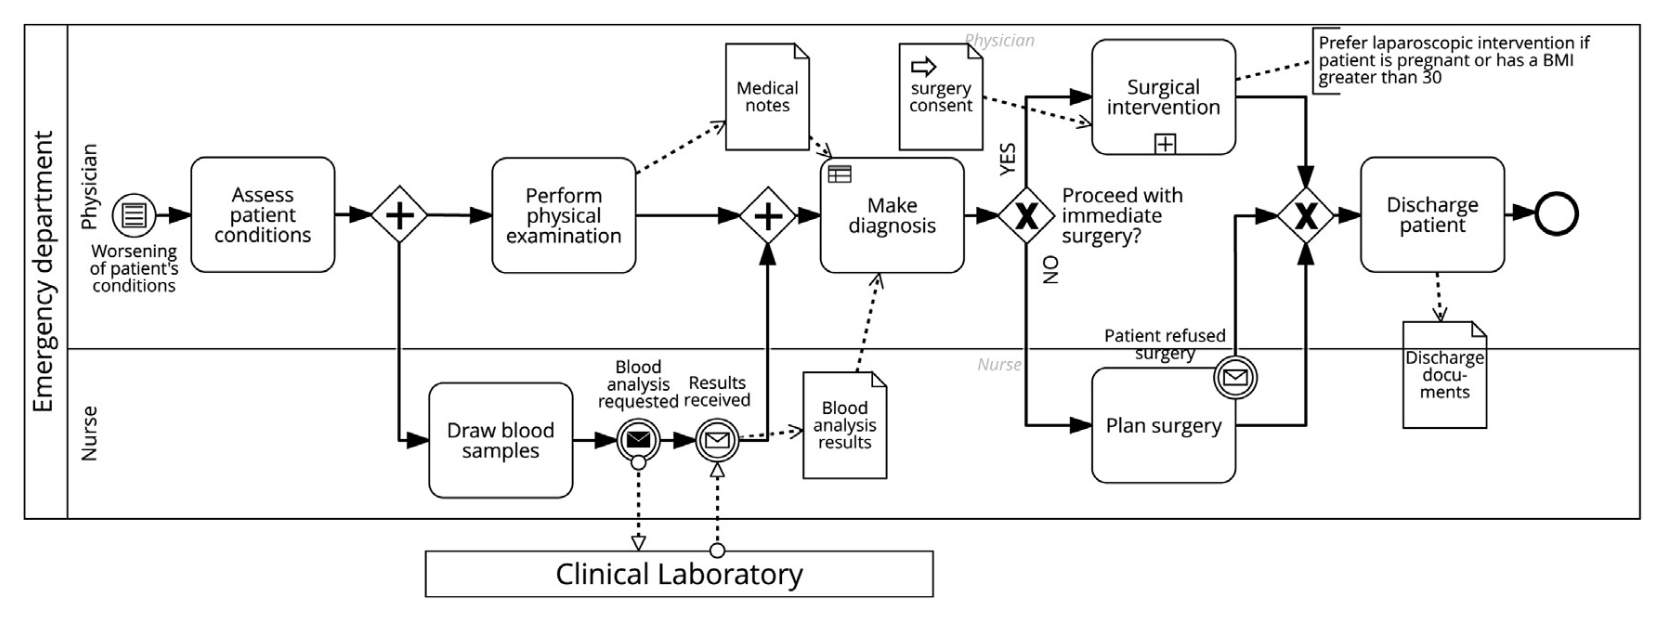
\includegraphics[width=\textwidth]{img/bpmn.png}
    \caption{Proceso simplificado de atención de urgencias en forma de diagrama de procesos BPMN. Fuente : \citetitle{pufahl_bpmn_2022}}
    \label{fig:bpmn}
\end{figure}

La Fig. 1 muestra una versión simplificada de un proceso de atención de urgencias, que se desencadena por un empeoramiento de las condiciones del paciente. Como primera tarea, el médico evalúa las condiciones del paciente.

A continuación, mientras realiza la exploración física, una enfermera extrae sangre al paciente. Las muestras de sangre se envían al laboratorio clínico para su análisis y, una vez listos, los resultados se envían de vuelta al servicio de urgencias. Con las notas de la exploración y los resultados del análisis de sangre, el médico tiene que hacer un diagnóstico. En función de los resultados, el médico realiza inmediatamente una intervención quirúrgica o la enfermera la planifica para los días siguientes, teniendo en cuenta que el paciente también puede negarse a someterse a una intervención quirúrgica. En todos los casos, el paciente es dado de alta y se le entregan los documentos de alta. Los diagramas BPMN pueden representar el flujo de control, el flujo de datos y los aspectos organizativos de un proceso con los siguientes conceptos.

\begin{itemize}
    \item Los diagramas de proceso BPMN pueden representar el flujo de control de un proceso con actividades (por ejemplo, Realizar examen físico), eventos relevantes (por ejemplo, Recibir resultados) y flujos de secuencia que los conectan. Las puertas de enlace, representadas como rombos, se utilizan para controlar los flujos de secuencia y definir comportamientos paralelos y alternativos.
    \item Las actividades pueden ser atómicas (tareas) o compuestas (subprocesos). Las tareas (por ejemplo, Realizar un examen físico) representan unidades atómicas de trabajo, mientras que los subprocesos representan actividades compuestas, que pueden colapsarse para ocultar detalles (por ejemplo, Intervención quirúrgica). BPMN presenta distintos tipos de tareas con comportamientos inherentes diferentes. Por ejemplo, las tareas de reglas de negocio se utilizan para representar tareas de toma de decisiones (p. ej., tarea Realizar diagnóstico).
    \item Los eventos externos relevantes se muestran como eventos BPMN (por ejemplo, Empeoramiento de las condiciones del paciente), que capturan los desencadenantes del proceso a los que reacciona el proceso, como mensajes, señales, condiciones (por ejemplo, Empeoramiento de las condiciones del paciente, excepciones (por ejemplo, Paciente rechazó la cirugía) y salidas producidas por el proceso (por ejemplo, Análisis de sangre solicitado).
    \item Los datos y documentos relevantes utilizados o producidos por las actividades del proceso pueden representarse con la ayuda de objetos de datos (por ejemplo, Notas médicas) o almacenes de datos cuando los datos considerados son persistentes. Se pueden adjuntar anotaciones de texto a los elementos del flujo de control para mejorar su descripción, como la anotación ''Prefer laparoscopic [...]'' asociada al subproceso Intervención quirúrgica.
    \item Las interacciones entre organizaciones pueden mostrarse mediante el concepto de pools (cada uno de ellos propietario de un proceso) (por ejemplo, el servicio de Urgencias y el laboratorio clínico) y un flujo de mensajes entre ellos.
    \item Los carriles de las agrupaciones (por ejemplo, la Enfermera y el Médico) pueden utilizarse para representar diferentes roles o sistemas que ejecutan las actividades incluidas.
\end{itemize}
